\section{Findings}
\todo{we might need to adjust this main table a bit -- it is exceeding the width of the page now}
\small
\begin{longtable}{|p{0.7cm}|p{5cm}|p{2.5cm}|p{3cm}|p{2.5cm}|}
\hline
\textbf{\#} & \textbf{Design Challenge} & \textbf{Worker Priority} & \textbf{Task Designer Priority} & \textbf{Platform Priority}\\
\hline
\endhead
[1] & \textbf{Platform Signup:} Setting expectations for worker protection & Platforms' protection from sensitive tasks & Large and diverse worker population & Liability protection \\
\hline
\multirow{2}{*}{[2-3]} & \textbf{Participation Preferences (Agency):} Defining boundaries for accepting tasks & To have diverse options for tasks & Large and diverse worker population & Limit participation for worker protection \\
 & \textbf{Participation Preferences (Awareness):} Supporting worker self-awareness & Self-awareness of triggers & Trust workers know what they can't do & Scaffold worker self-awareness \\
\hline
\multirow{3}{*}{[4-6]} & \textbf{Decision to Participate (Warning):} Warning workers without deterring participation & Information to decide to opt-in or not to task & Convince workers to do the task & Worker and task designer retention \\
 & \textbf{Decision to Participate (Definition):} Ensuring shared definitions of content & Clear definition of content & Autonomy in describing risk & Provide definition in compliance to regulations and policies \\
 & \textbf{Decision to Participate (Accountability):} Balancing task designer autonomy with agency & Consequences for failed risk disclosure & Agency to disclose risk & Mechanism to resolve disputes \\
\hline
\multirow{2}{*}{[7-8]} & \textbf{Task Completion (Consent):} Balancing task completion with freedom to stop & Stop task if uncomfortable & Full worker task completion & Prevent task abandonment at scale \\
 & \textbf{Task Completion (Payment):} Fair pay for RAI content work & More payment for difficulty and well-being harm & Quality worker performance & Optimize labor costs while retaining workers \\
\hline
\multirow{2}{*}{[9-10]} & \textbf{Post-task Completion (Feedback):} Encouraging quality feedback & Choice to give feedback & Quality feedback & Large scale quality feedback \\
& \textbf{Post-task Completion (Redress):} Mitigating harms from failed risk disclosure & Response from task designers & Make up for mistakes & Maintain trust in platform \\
\hline
\end{longtable}
\normalsize


% \small
% \begin{longtable}{|p{0.5cm}|p{5cm}|p{3cm}|p{3cm}|p{3cm}|}
% \hline
% \textbf{\#} & \textbf{Design Challenge} & \textbf{Worker Priority} & \textbf{Task Designer Priority} & \textbf{Platform Priority}\\
% \hline
% \endhead
% [\#1] & \textbf{Platform Signup:} Setting expectations for worker protection & Platforms' protection from sensitive tasks & Large and diverse worker population & Liability protection \\
% \hline
% [\#2] & \textbf{Participation Preferences (Agency):} Defining boundaries for accepting tasks &  To have diverse options for tasks & Large and diverse worker population & Limit participation for worker protection\\
% \hline
% [\#3] & \textbf{Participation Preferences (Awareness):} Supporting worker self-awareness &  Self-awareness of triggers & Trust workers know what they can't do & Scaffold worker self-awareness\\
% \hline
% [\#4] & \textbf{Decision to Participate (Warning):} Warning workers without deterring participation & Information to decide to opt-in or not to task & Convince workers to do the task & Worker and task designer retention\\
% \hline
% [\#5] & \textbf{Decision to Participate (Definition):} Ensuring shared definitions of content &  Clear definition of content & Autonomy in describing risk & Provide definition in compliance to regulations and policies\\
% \hline
% [\#6] &\textbf{Decision to Participate (Accountability):} Balancing task designer autonomy with agency & Consequences for failed risk disclosure & Agency to disclose risk & Mechanism to resolve disputes\\
% \hline
% [\#7] &\textbf{Task Completion (Consent):} Balancing task completion with freedom to stop & Stop task if uncomfortable & Full worker task completion & Prevent task abandonment at scale\\
% \hline
% [\#8] &\textbf{Task Completion (Payment):} Fair pay for RAI content work & More payment for difficulty and well-being harm & Quality worker performance & Optimize labor costs while retaining workers\\
% \hline
% [\#9] & \textbf{Post-task Completion (Feedback):} Encouraging  quality feedback & Choice to give feedback & Quality feedback & Large scale quality feedback \\
% \hline
% [\#10] & \textbf{Post-task Completion (Redress):} Mitigating harms from failed risk disclosure & Response from task designers & Make up for mistakes &  Maintain trust in platform\\
% \hline
% \end{longtable}
% \normalsize

% \todo{Hong: A few high-level thoughts: (1) we can cluster some challenges together based on stages and how you organize your findings (10 row is a bit too dense for one single table). For example, we can cluster 1-3 as signup and preferences; 4-8 as participation and completion; 9-10 as post-task completion. Alternatively, we can create a few subtables (2) Is it better to name challengs as "design challenges" more specifically to surface our theme "disclosure as a design challenge"? Also make sure that you refer them back in your findings? (3) "worker need" feels a bit odd as this is not about "need finding"? how about "worker priorities/perspectives" and so forth?(4) some design tensions here seem to be more generic than risk specific (and have been covered by previous literatur?) for example tension \#8? Suggest to either remove them or contextualize them even more in your data to bring out the novelty here }


\subsection{Platform Signup}
% note for my co-authors here is the structure I'm trying to follow for each section:
% 1 -- describe the challenge from each perspective
% 2 -- describe proposed solutions (this is where I can bring in references to our probes or hypothetical/higher-level solutions)
% 3 -- describe issues with the proposed solutions
\subsubsection{Setting expectations for worker protection}
Although platforms sometimes provide opt-in or opt-out options for sensitive content, workers emphasized that platforms should be accountable for enforcing these protections, even if platforms may struggle to guarantee full shielding from harm. When asked whether they were prompted about their tolerance for sensitive content upon first joining a platform, few could recall such questions. After being shown an example of how a platform might ask about willingness to view sensitive content (see Figure \ref{fig:participation-survey}), workers expressed two main sentiments. First, some, like W1, noted that platforms should actively uphold the preferences workers indicate: \textit{``I think the platform should protect [us]. [If a worker] wants to say no [and they] don't want to see [sensitive content]. It shouldn't be popping up anymore''} (W1). 

\begin{figure}[htbp]
    \centering
    \includegraphics[width=\textwidth]{figures/study-probes/participation_survey.pdf}     
    \caption{Participation survey probe}
    \label{fig:participation-survey} 
\end{figure}

Other workers, such as W11, felt it was acceptable for platforms to at least offer an explicit opt-in option for viewing sensitive content, reflecting that \textit{``from the frequency of the things I've been seeing I would say it's almost impossible for you to [not] be exposed to explicit contents \dots so I think it's okay [for the platform to be] vouching that you will not see [the content]''} (W11). However, W11 later indicated that if questions were instead more specific--for example, asking about willingness to view racist content--it would be more important to enforce worker preferences, as they were personally harmed by that specific type of content (W11). From the platform perspective, P1 explained that such opt-in statements \textit{``gives the company or the employer some cover''}, but suggested that support the platform offers \textit{``could be more comprehensive. It could offer resources. You can say `if you experience issues, please reach out to us''} (P1). These findings surface a recurring tension: while workers expect platforms to uphold accountability when presenting opt-in or opt-out options, platforms face legal challenges in guaranteeing that workers will never see sensitive content.
 
\subsection{Participation Preferences}
\subsubsection{Defining boundaries for task participation}
We found that while platforms sometimes restrict sensitive tasks to certain workers, some task designers prefer input from diverse groups. For example, P1 described an instance where their platform restricted tasks on self-harm to an `expert' population, defined as adults familiar with how self-harm could be encouraged by a specific AI system in a given domain (P1). P1 went on to explain that experts may be better equipped for exposure to such content: \textit{``if someone works in counter terrorism, they're more readily [prepared]. I definitely think that they are a more prepared audience for dealing with the kind of content that might be [encountered]''} (P1). This desire to limit participation, however, conflicts with prior literature that emphasized the importance of diverse perspectives in responsible AI development~\cite{qian2025locating, dalal2024provocation}. This was further validated by several task designers in our participant pool (e.g., T8 and T7) who expressed the need for a diverse samples. 

These tensions became particularly pronounced when we discussed the idea of workers being allowed to filter tasks that contained certain types of sensitive content. Some task designers strongly expressed a concern about participation in their tasks being limited. T3 describes this tension:
\begin{quote}
    \textit{``[From a] researcher's perspective, you [will] begin to see that if a lot of people are actually turning on the sensitive [content filter so they don't see these tasks. Then you start to see a reduction in study participants, and at the end of the day, you might not be able to get enough [participants] \dots [From] the workers' perspective,  a lot of them would most likely turn [the filter] on.''} -T3
\end{quote} 
One of the problems task designers had with the idea of a task filter was with how broad the definition of content that was filtered was. For example, T14 observed that task filters for a categorization of ``sensitive content'' may be too broad: \textit{``[the task] might be sensitive, but not as sensitive as a worker might imagine it to be [by] filtering it out, they don't get to work on it''} (T14). A few task designers offered suggestions to resolve this tension. For example, T2 suggested that rather than a broad categorization, workers are given \textit{``a bit of control, like [with an option to indicate] words that you don't want to see''} (T2).


\begin{figure}
    \centering
    % Top row: Two images side-by-side
    \begin{subfigure}[b]{0.48\textwidth}
        \centering
        \includegraphics[width=\textwidth]{figures/study-probes/task-filters/AI-task-filter.pdf} 
        \caption{AI task filter}
    \end{subfigure}
    \hfill
    \begin{subfigure}[b]{0.48\textwidth}
        \centering
        \includegraphics[width=\textwidth]{figures/study-probes/task-filters/category-task-filter.pdf} 
        \caption{Category task filter}
    \end{subfigure}
    \vspace{1em} % Add space between rows
    % Bottom row: One image
    \begin{subfigure}[b]{0.98\textwidth}
        \centering
        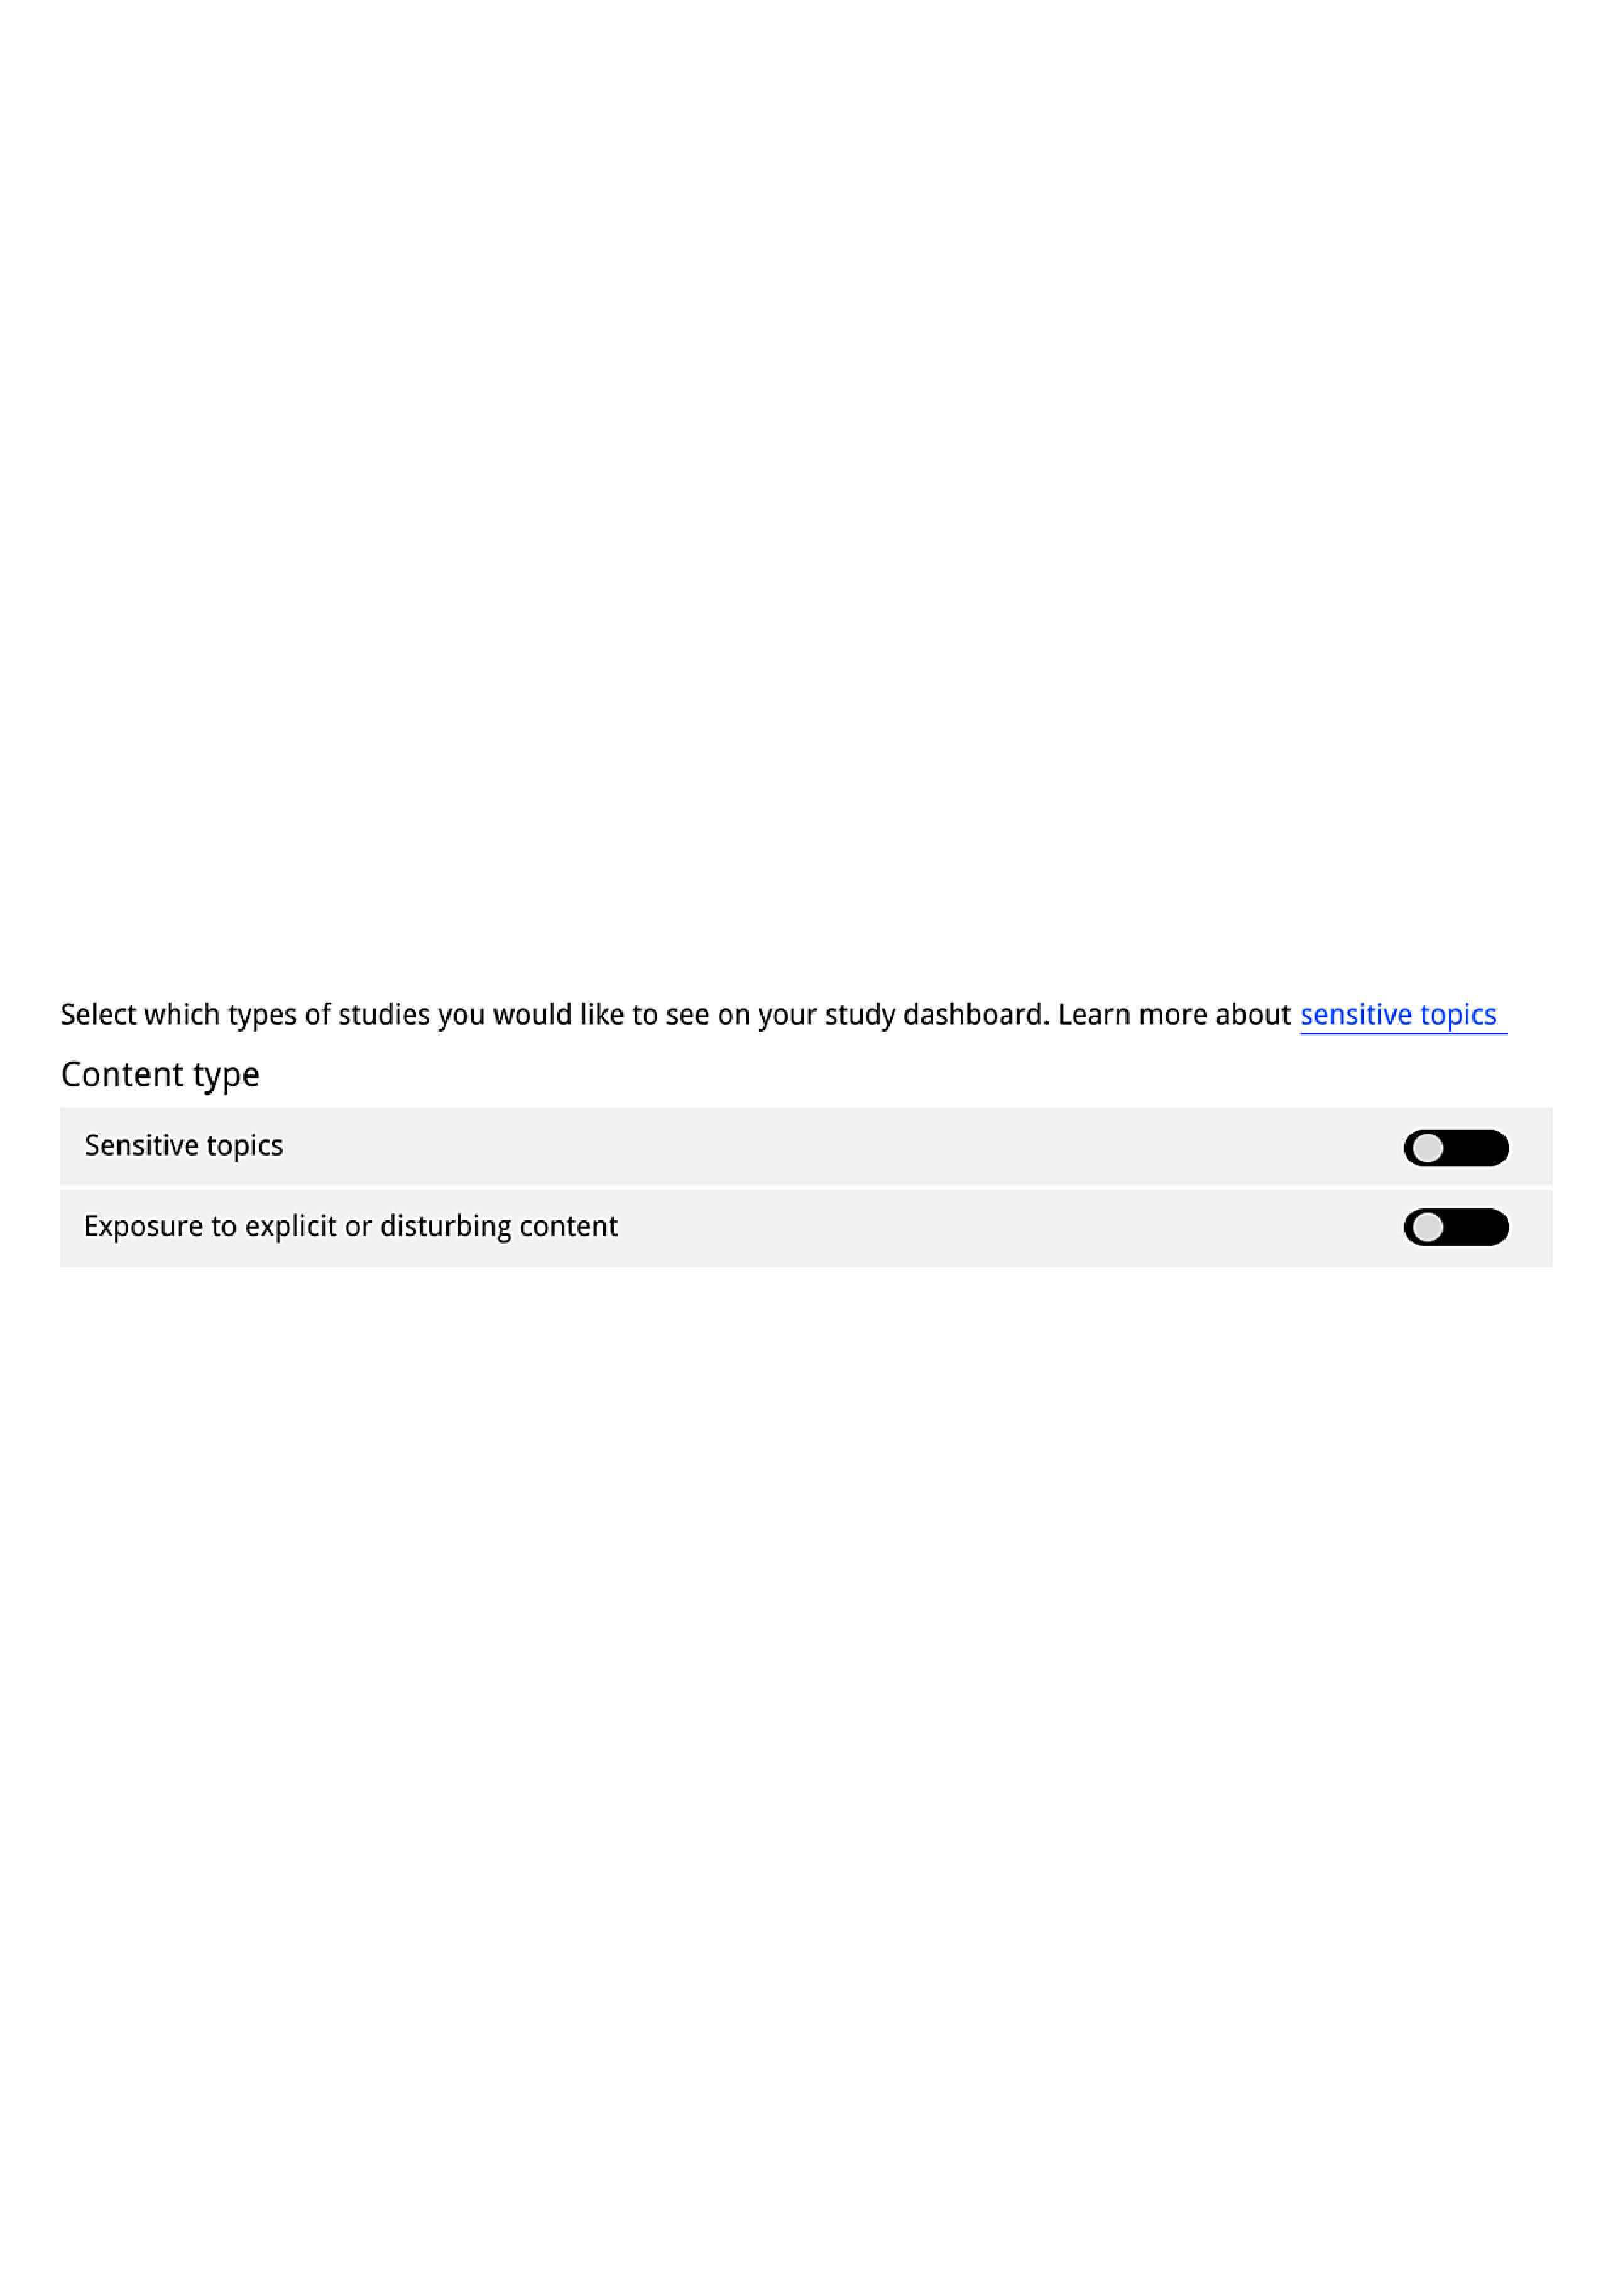
\includegraphics[width=0.6\textwidth]{figures/study-probes/task-filters/toggle-task-filter.pdf}
        \caption{Toggle two-category task filter}
    \end{subfigure}
    \caption{Worker task filters}
    \label{fig:worker-task-filters}
\end{figure}

When we presented a range of options, from generic task filters to specific options for workers, participants expressed mixed preferences. Some workers echoed concerns that task filters could limit the number of tasks available and preferred instead to decide on a case-by-case basis using task warnings (W2, W3, and W9). Others favored category-specific filters (W5). On the other end of the spectrum, a few workers expressed they were not concerned about reduced task availability, stating \textit{``it's not really going to be much of an issue \dots as much as I care about the job, you know, I still have to take good care of myself. I don't want something that will probably affect [my] mental health in any way''} (W10). Ultimately, our findings surface a key tension: while restricting participation in tasks either by a platform or through worker preference can protect workers from exposure, it must also take into account workers' desires to view tasks they're interested in and task designers' needs to sustain participation. 

\subsubsection{Supporting worker self-awareness}
Another tension around task filters concerned whether workers were fully aware of what types of content upset or ``triggered'' them. Many task designers assumed that most workers could reliability identify their boundaries. For instance, T15 reflected that if a worker completed RAI content work tasks for about a week, they would be familiar enough with the content to be able to indicate what upsets them. Many workers expressed a similar sentiment that they knew what specific content could upset them. For example, W3 explained that they have never liked seeing violence, while W6 stated they never want to do tasks involving sex exploitation. 

We learned, however, that not all workers were certain of their limits. On the task designer side, T15 later expressed a concern that \textit{``doing this type of work can be a little numbing, and workers may not be paying the best attention to their own well-being''} (T15). This concern was justified as some  workers reflected on how they had become accustomed to viewing harmful content over time (e.g., T5, W10). As W10 explained, \textit{``right about now, I'm used to reviewing and working on this kind of task''} (W10). Moreover, some workers, like W6, had to view a task that displayed a violent altercation to realize they never wanted to complete tasks that showed someone getting injured. Other participants explained that, regardless of whether they were aware of what upset them, they felt some workers just didn't care to protect their well-being: \textit{``I know for a fact that lot of people don't really care about [what's] sensitive or not \dots a lot of [workers] say they don't really care if [a task is] sensitive or not. They just want to do it and collect their money''} (W3). To address this, T15 suggested there could be design features to help workers be more \textit{``introspective''}. Here, we surface another tension:  not all workers are aware of their limits to harmful content, raising questions about how effectively they can use platform features like task filters to protect themselves.

\subsection{Decision to Participate}
\subsubsection{Warning workers without deterring participation}
A key concern held by task designers was that disclosing risk would deter workers from participating in their tasks. Indeed, we found that workers viewed warnings as a crucial component in how they make informed decisions to complete tasks. Several task designers feared that warning workers of their task's sensitive content would dissuade workers from enrolling in the task (T2). In this way, task designers in our study faced issues similar to those echoed in prior research in prioritizing obtaining task data over everything else ~\cite{qian2025locating, finnerty2013keep, kittur2008crowdsourcing}. Some task designers felt an ethical obligation to include at least some basic type of warning, despite their perceived risks to the quality and speed of data collection (e.g., T12). Moreover, some task designers argued that \textit{``people who try to be responsible will not worry about [having enough worker participation] because you always need to make sure that you accurately represent the task before worrying about task completion''} (T15). T2 also reflected that responsibility for participation in RAI content work should rest with the platform, not individual task designers: \textit{``that's for the platform to work on, because [we are] the customers [of] platform that [we're] using''} (T2). 

On the other side of the issue, some workers explained that disclosure of risk was not the only thing they considered when deciding whether to complete a task. For example, W2 explained they decide to do a task based on whether it's \textit{``fun''} while W3 expressed that the amount of payment is the most important factor for them. In contrast, other worker participants expressed that warnings for a task were crucial to help them make informed decisions about whether to do a task or not. For instance, W3 explained they decided whether or not to do tasks based on whether the description in the warning was something they could \textit{``stomach''} (W3). Other workers described a similar decision-making strategy (e.g., W4 and W6). As W9 summed up: 
\begin{quote}
    \textit{`` What I want to know about [a task] is [with the] images that will be shown, what they actually contain. [If] \dots it's a task like I feel I wouldn't be comfortable [with] \dots You know, in the end, I'm also a human being. As I'm training the model, I have to consider my own personal [preferences] also. So if it's something I feel I'll be able to work with, I'll proceed to work on it.''} -W9
\end{quote}
Moreover, some workers described experiences where the disclosure of risk was insufficient, resulting in them being greatly negatively impacted. W6 described an instance when they decided not to finish after a task because they found the content was too \textit{``brutal''} to continue. 
% W1 expressed a similar sentiment, stating that \textit{``at least I have to be notified''} of the risks in the task (W1). 
To mitigate this problem, P2 suggested that platforms offer an estimate of how frequently workers may view content, telling workers \textit{``your likelihood of seeing [a type of harmful content] is 1 in 100 \dots Putting numbers, averages, and percent likelihoods behind [warnings] would be helpful \dots [and] would help [platforms] get more people doing the work''} (P2). Moreover, P2 proposed that platforms may offer workers alternatives to RAI content work tasks as a tradeoff: 
\begin{quote}
    \textit{`` if you answer this harmful question, you get paid more, but if you decide not to, we will give you five extra non-harmful questions so that [workers] have the option of: `do you want to expose yourself to harm and get paid the same and do less work or get paid the same and do more work?'''} - P2
\end{quote}
Importantly, P2's suggestions assumed that platforms could provide non-RAI content tasks. Given worker observations of platforms increasingly offering more RAI content worker tasks (e.g., W11), it is unclear how feasible such options would be in practice. 
This theme surfaces a key tension: task designers were often hesitant to provide detailed warnings out of fear they might deter participation, while workers viewed risk disclosure as crucial to their decision-making process. Platform representatives offered initial suggestions on different ways in which platforms can address this challenge through warnings or other strategies. 

\subsubsection{Ensuring shared definitions of sensitive
content}
Another aspect we observed across the three groups of participants was that of discrepancies in how content should be involved in risk disclosure (e.g., `sensitive content') and how it should be defined.
Some task designers made an assumption that their definition of risky, sensitive, or explicit content was aligned with others' to the point where they didn't need to read platform definitions. For example, T15 \textit{``very rarely''} read platform definition of sensitive content because they \textit{``intuitively know the type of content that\'s in there''} and the \textit{``platform typically would put [a] blanket statement \dots [that's] usually not useful to read''} (T15). However, when prompted to explain how they personally defined `sensitive' versus `explicit or disturbing' content, the explanations that several participants provided varied widely. Some participants interpreted sensitive topics as \textit{``private information [about workers]''} (T1), while other participants viewed sensitive content as certain topics that may trigger some workers and be neutral for others. For example, T11 determined \textit{``cyber bullying is sensitive because it triggers [you] if you've been cyberbullied before''} (T11). Moreover, T5 defined sensitive content based on examples of viewer discretion warnings they saw on television: \textit{``[in] movies on Netflix \dots there's always a warning that says `nudity or violence and drugs'''} (T5). These findings echo longstanding debates about how many decisions in content moderation are left to \textit{`I know it when I see it'} judgments~\cite{gillespie2020expanding, ohioknow}.

Because definitions of sensitive content are subjective and inconsistent, differences between the task designers' and the workers' perceptions could undermine the effectiveness of warnings. 
W1 illustrated an instance where differing definitions of content necessarily for risk disclosure negatively affected them as workers: \textit{``maybe to [the task designer who] posted it \dots there is nothing that sensitive. But then [for the worker] doing it, I see it as a sensitive issue that [the worker] doesn't want to see''} (W1). As W5 emphasized, a shared definition of the severity of the task can tell workers that the task \textit{``is going to be deeply harmful or offensive''} (W5). Platform representatives described using commonly known taxonomies of harm (P1) to define risks to workers. Additionally, P2 explained that it is a priority for platforms to base definitions of content categories on existing regulation and policy, such as the European Union's Digital Services Act~\cite{EU-DSA-2022}.


% A potential solution is to provide AI-generated suggestions about warnings. For T5, feedback about what warnings other task designers have used in similar tasks \textit{"gives [T5] the instinct that this is bad and this is not"}(T5). 
\subsubsection{Balancing task designer agency with
need for accountability}
\begin{figure}[htbp]
    \centering

    % First row
    \begin{subfigure}[b]{0.5\textwidth}
        \centering
        \includegraphics[width=\textwidth]{figures/study-probes/task-designer-probes/binary-task-designer.pdf}
        \caption{Binary}
        \label{fig:manual-binary}
    \end{subfigure}
    \hfill
    \begin{subfigure}[b]{0.48\textwidth}
        \centering
        \includegraphics[width=\textwidth]{figures/study-probes/task-designer-probes/keywords-task-designer.pdf}
        \caption{(Keywords}
        \label{fig:manual-keywords}
    \end{subfigure}

    \vspace{0.5em}

    % Second row
    \begin{subfigure}[b]{0.48\textwidth}
        \centering
        \includegraphics[width=\textwidth]{figures/study-probes/task-designer-probes/category-task-designer.pdf}
        \caption{Category}
        \label{fig:manual-category}
    \end{subfigure}
    \hfill
    \begin{subfigure}[b]{0.48\textwidth}
        \centering
        \includegraphics[width=\textwidth]{figures/study-probes/task-designer-probes/modality-task-designer.pdf}
        \caption{Modality}
        \label{fig:manual-modality}
    \end{subfigure}

    \vspace{0.5em}

    % Third row
    \begin{subfigure}[b]{0.48\textwidth}
        \centering
        \includegraphics[width=\textwidth]{figures/study-probes/task-designer-probes/severity-task-designer.pdf}
        \caption{Severity}
        \label{fig:manual-severity}
    \end{subfigure}
    \hfill
    \begin{subfigure}[b]{0.48\textwidth}
        \centering
        \includegraphics[width=\textwidth]{figures/study-probes/task-designer-probes/example-task-designer.pdf}
        \caption{Example}
        \label{fig:manual-example}
    \end{subfigure}
    \caption{Task designer manual options}
    \label{fig:task-designer-manual}
\end{figure}


\begin{figure}[htbp]
    \centering
    % Top row
    \begin{subfigure}[b]{0.48\textwidth}
        \centering
        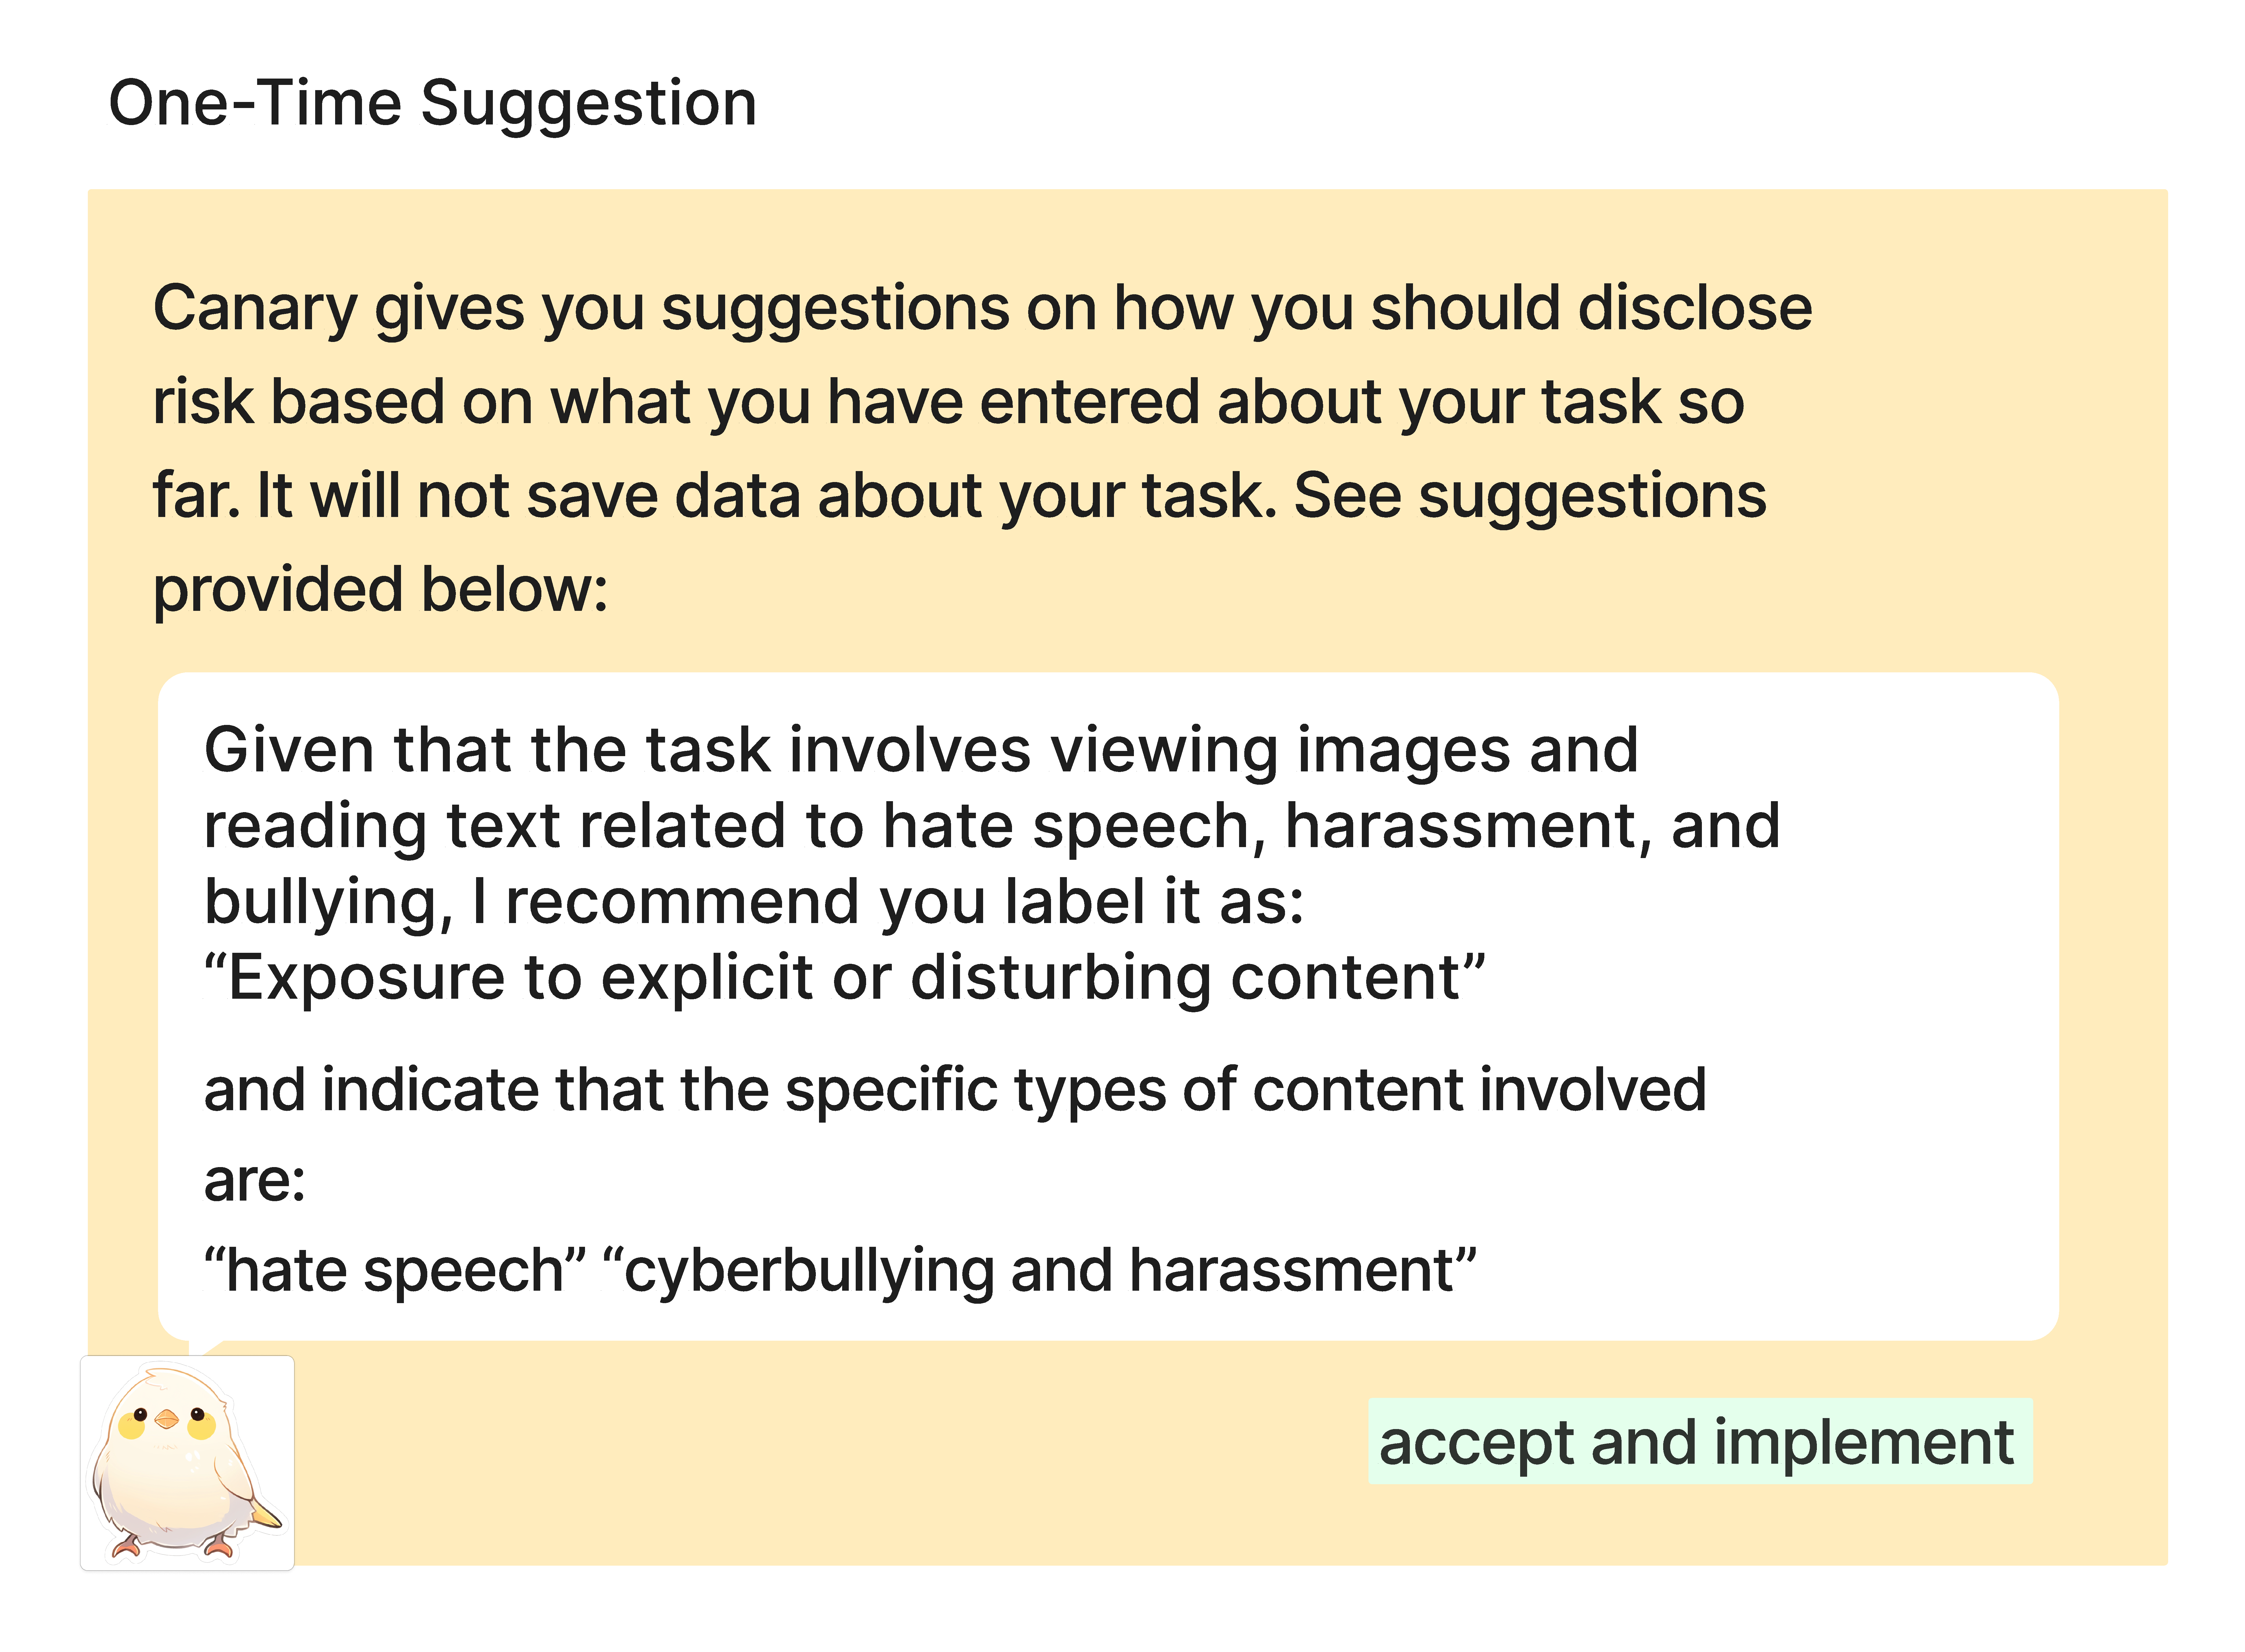
\includegraphics[width=\textwidth]{figures/study-probes/AI-probes/AI-one-time.pdf}
        \caption{Generic AI suggestion\protect\footnotemark}
        \label{fig:AI-generic}
    \end{subfigure}
    \hfill
    \begin{subfigure}[b]{0.48\textwidth}
        \centering
        \includegraphics[width=\textwidth]{figures/study-probes/AI-probes/AI-explanation.pdf} 
        \caption{AI suggestion with explanation}
        \label{fig:AI-explanation}
    \end{subfigure}
    \vspace{1em} % Space between rows
    % Bottom row
    \begin{subfigure}[b]{0.48\textwidth}
        \centering
        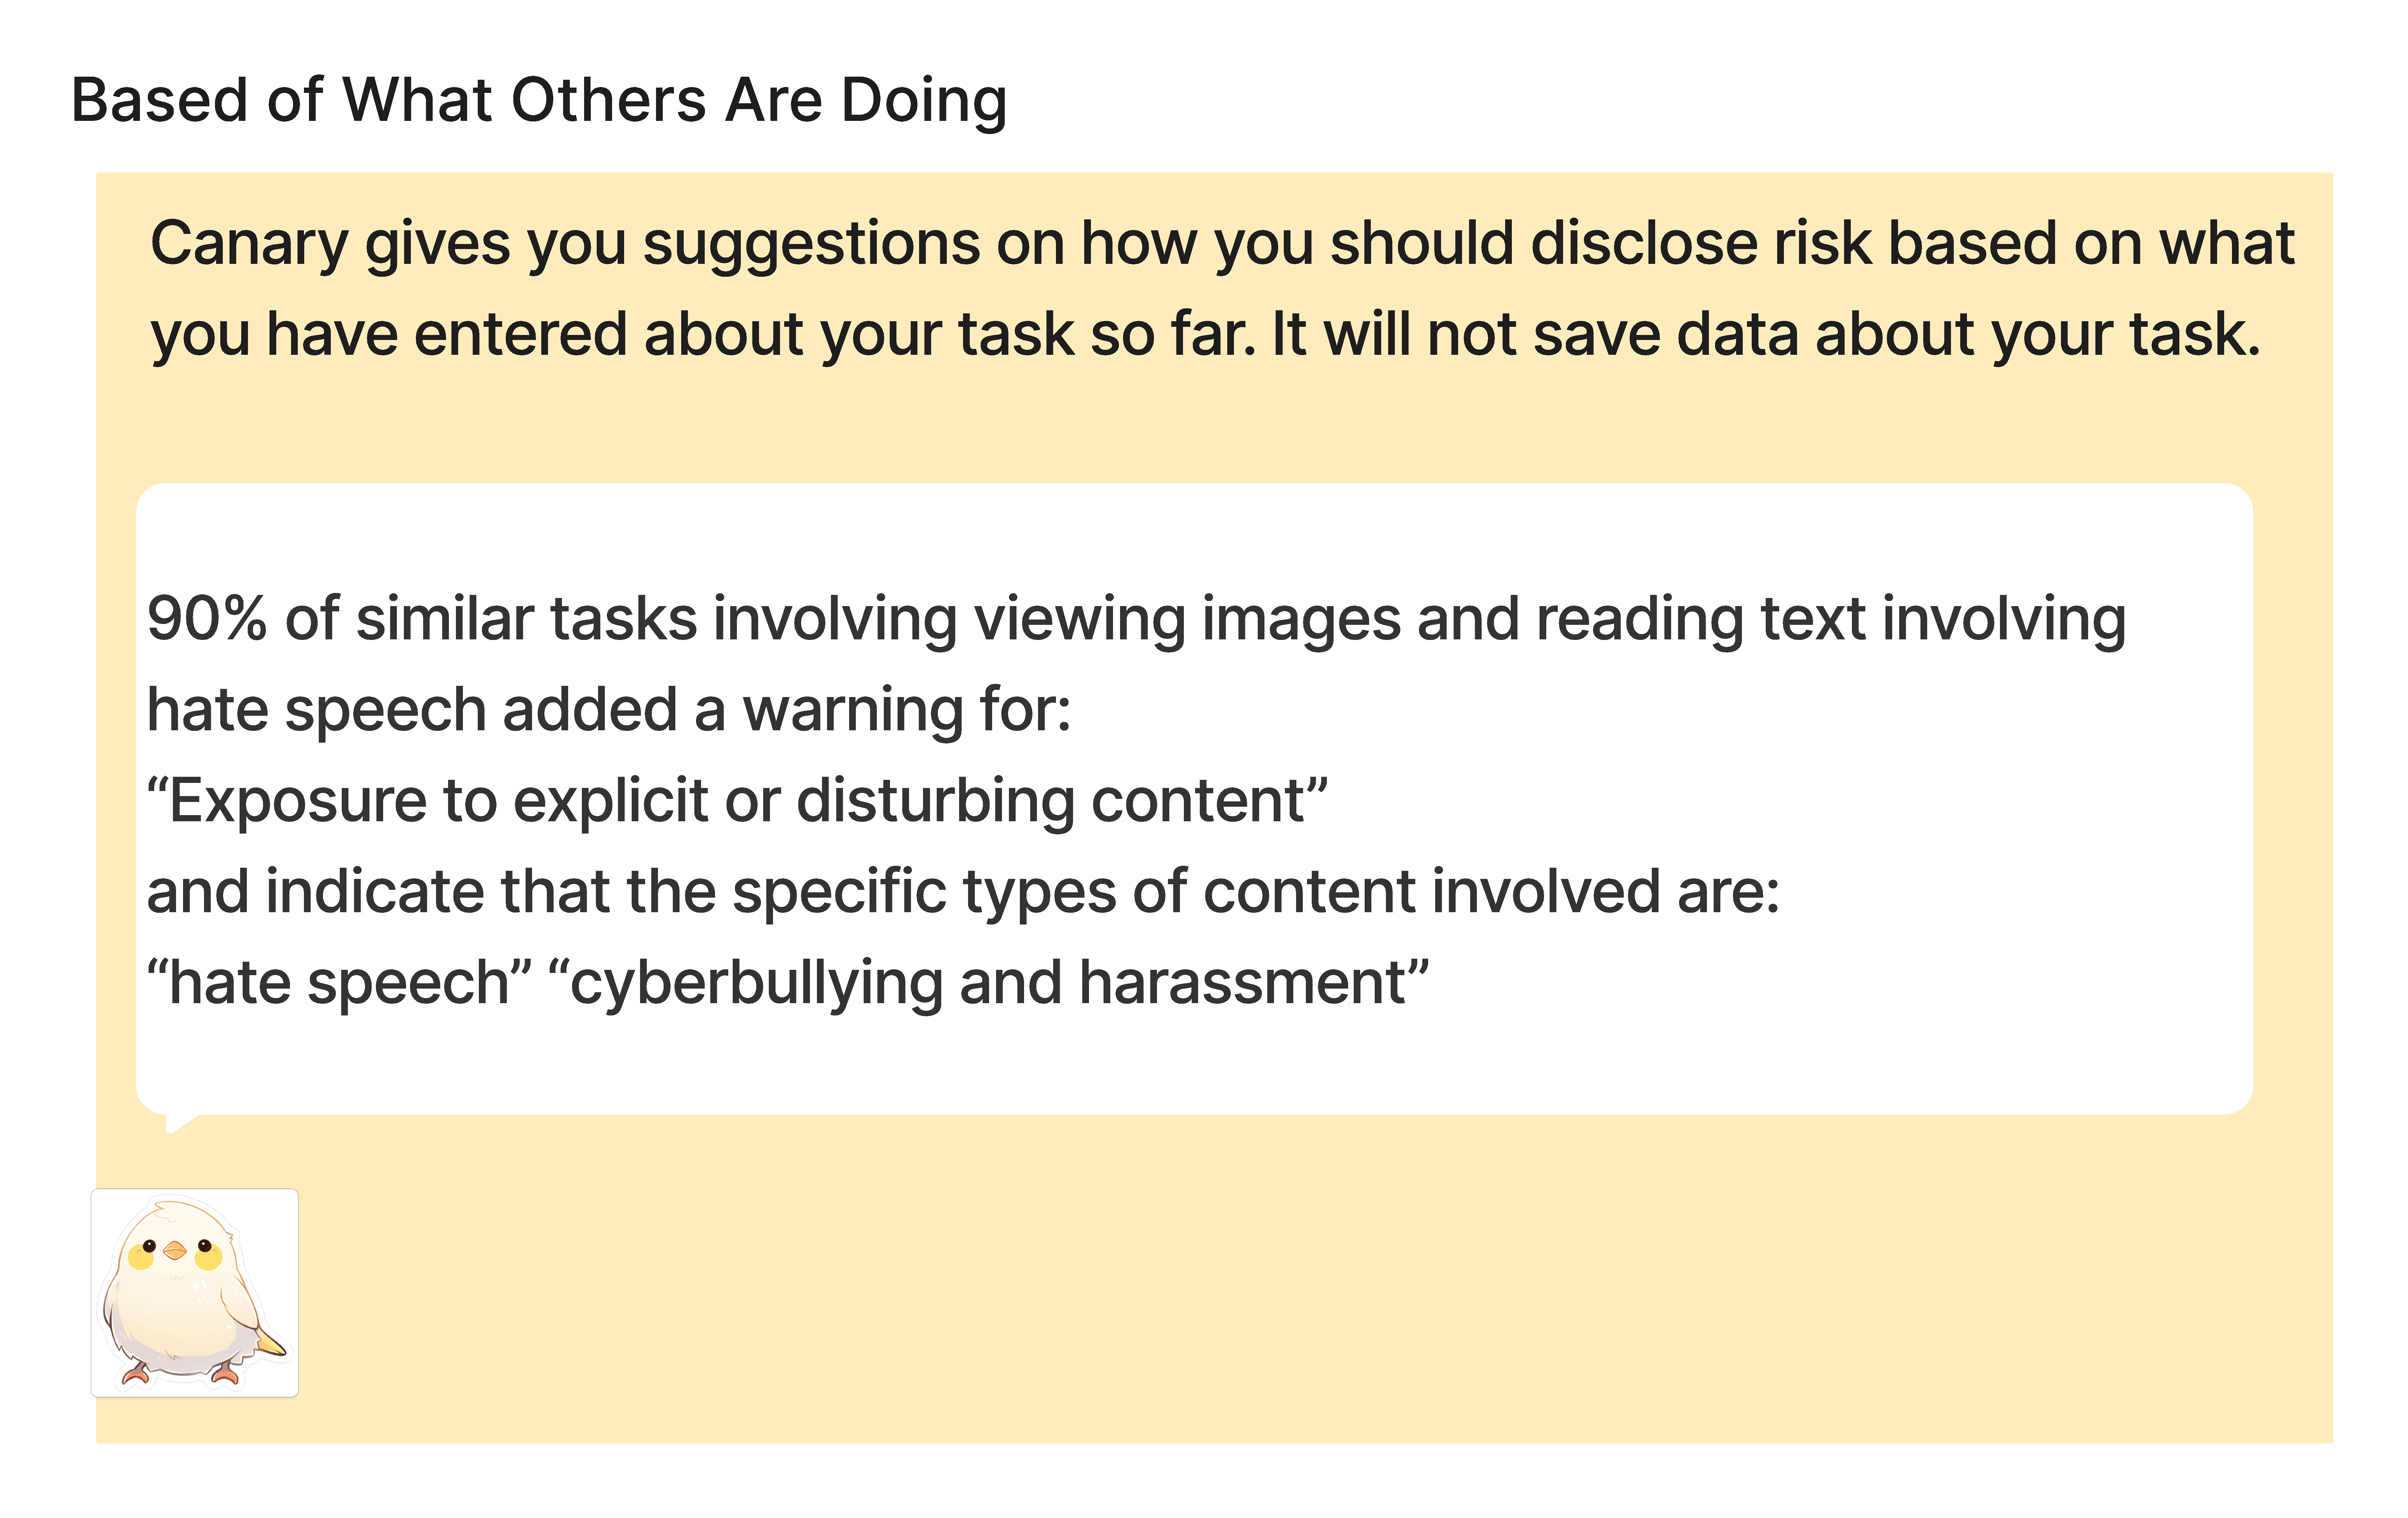
\includegraphics[width=\textwidth]{figures/study-probes/AI-probes/AI-task-designers.pdf}
        \caption{Suggestion based on what other task designers have done}
        \label{fig:AI-based-on-others}
    \end{subfigure}
    \hfill
    \begin{subfigure}[b]{0.48\textwidth}
        \centering
        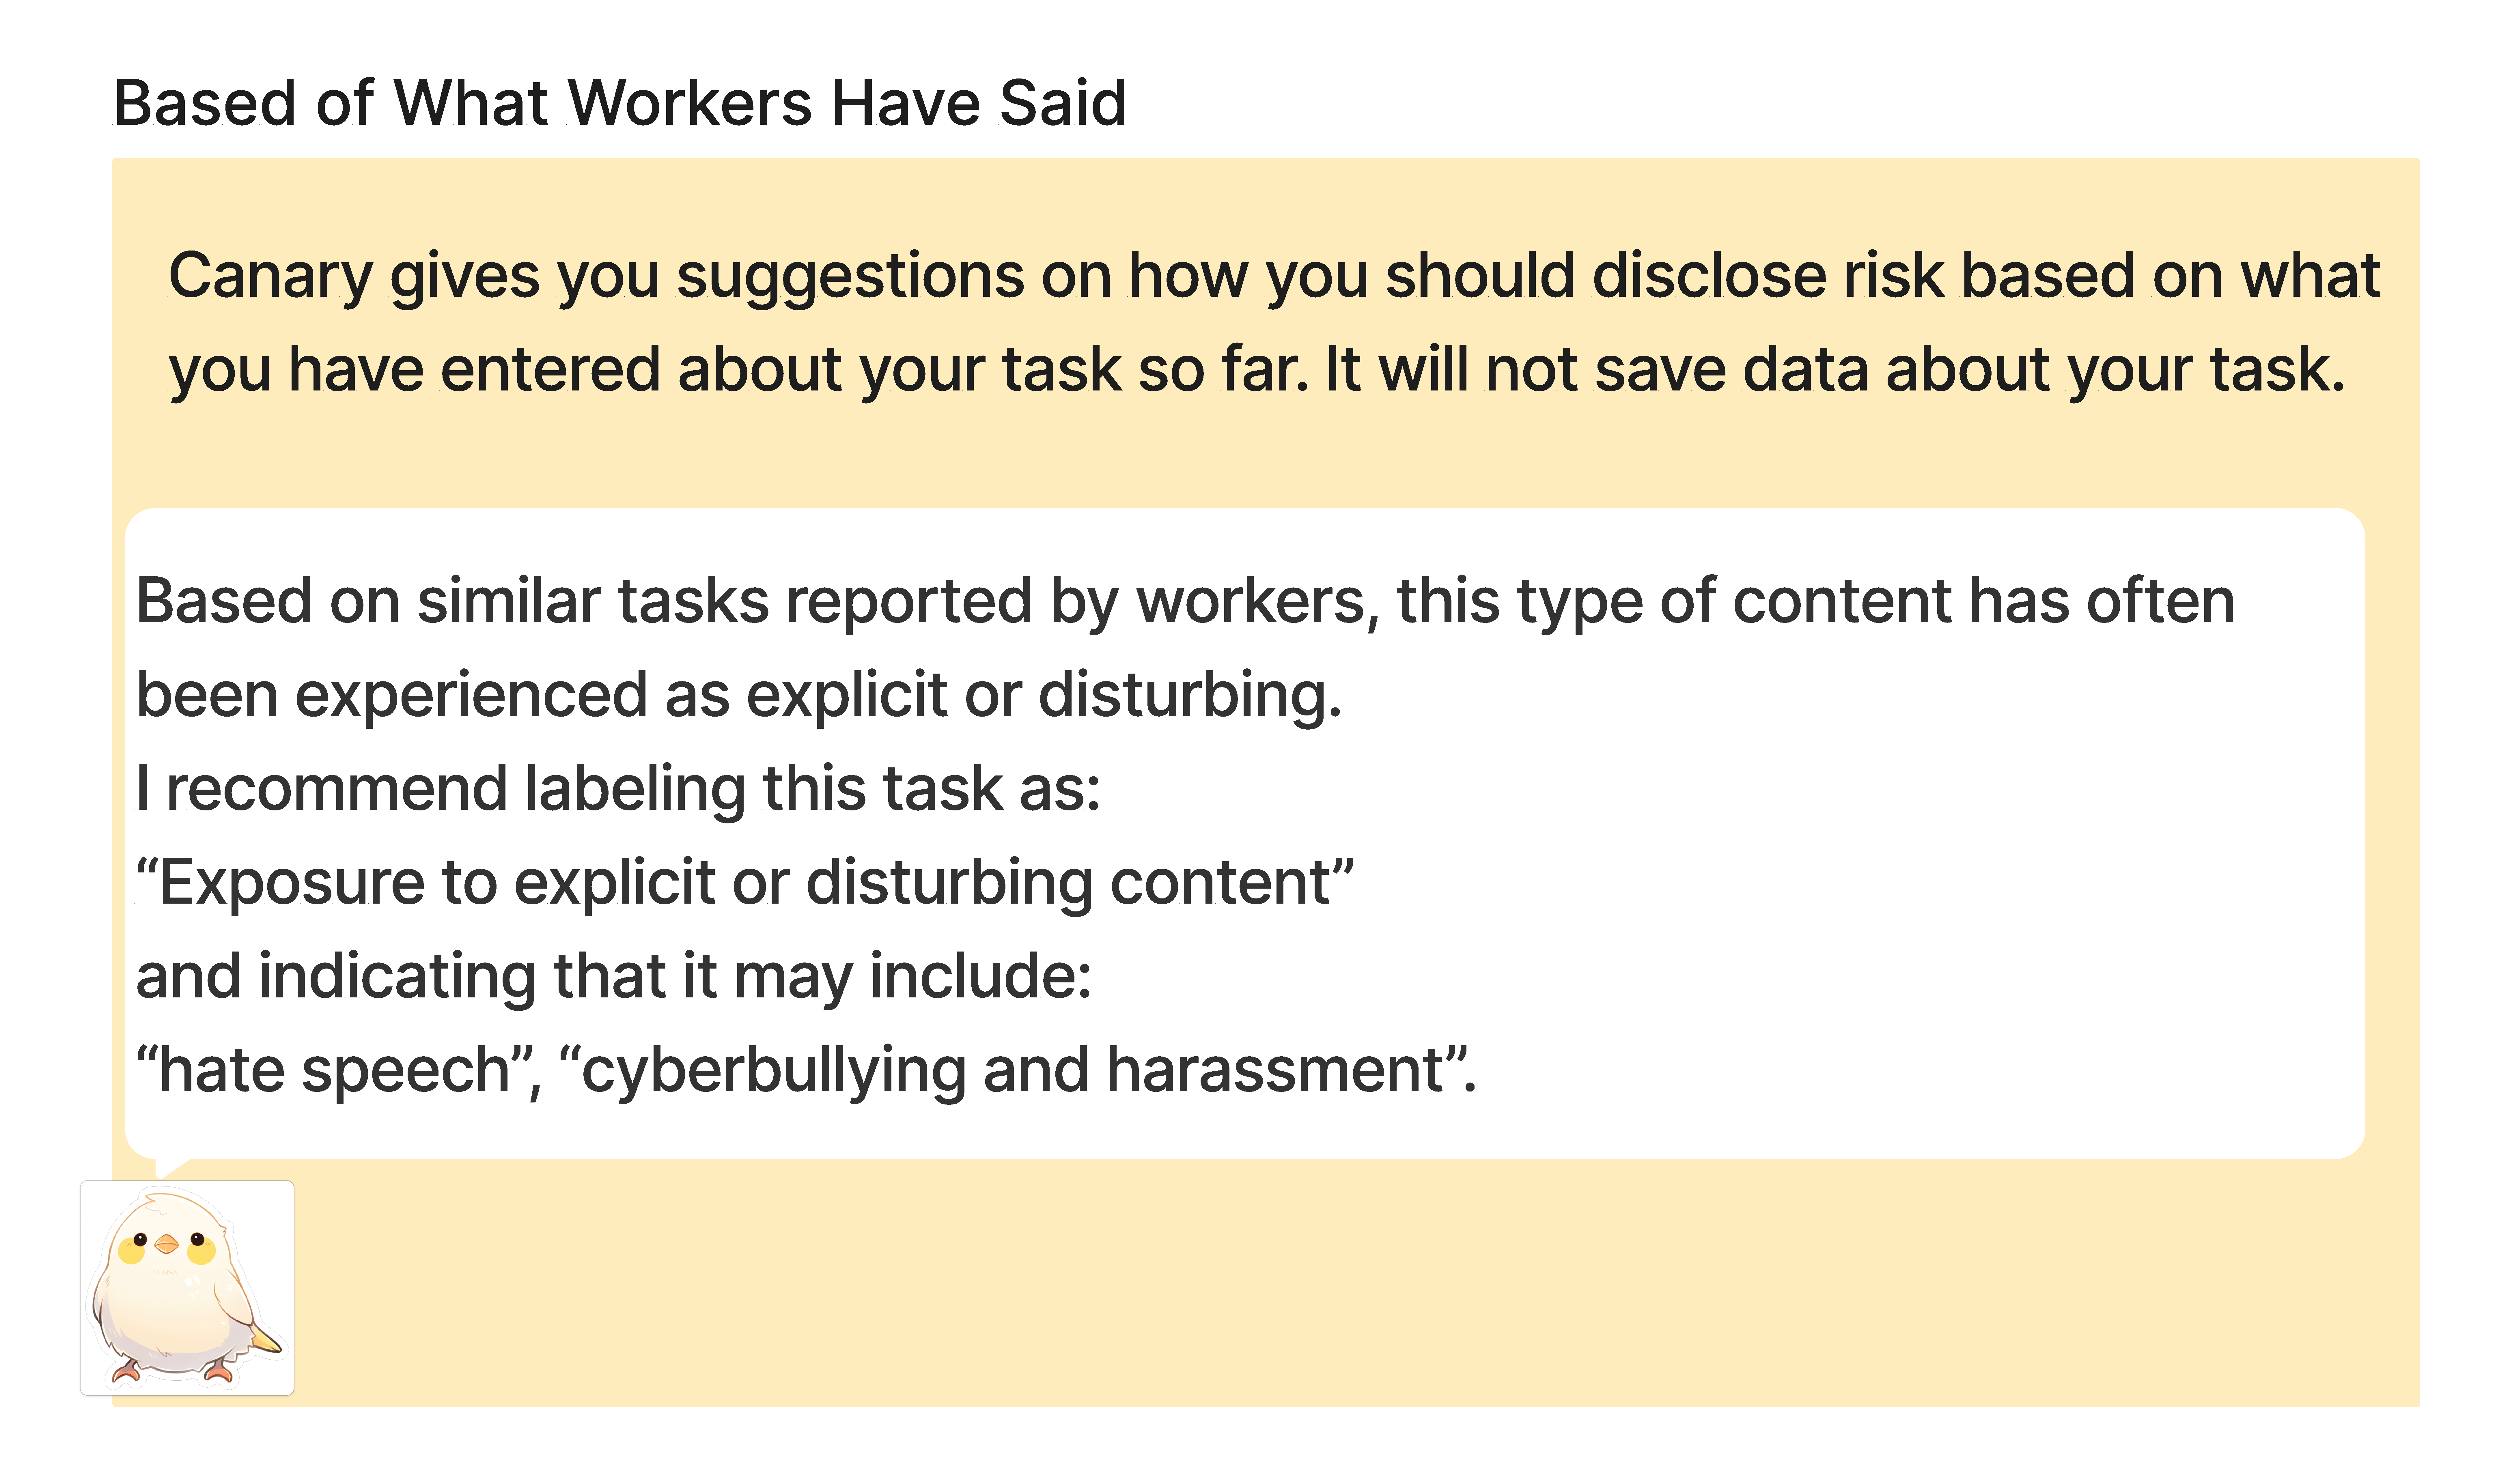
\includegraphics[width=\textwidth]{figures/study-probes/AI-probes/AI-workers.pdf} 
        \caption{Suggestion based on what workers have said}
        \label{AI-based-on-workers}
    \end{subfigure}
    \caption{AI warning suggestions}
    \label{fig:task-designer-AI}
\end{figure}

\footnotetext{Icon credit: https://wallpapers-clan.com/sticker-png/cute-canary-bird}

% challenge 
Another key tension we found was in task designers' desire for agency in determining how risk should be disclosed for these tasks, with workers' desire for accountability mechanisms to be in place to prevent instances of inadequate risk disclosure. Several task designers indicated that they wanted agency to make the final decisions about how to disclose risk in their tasks. As T1 explained: \textit{``I know everything about my research, and I want to explain my research by my word[s] and by myself''} (T1). Other participants were open to receiving additional support in determining what warnings were most appropriate for their tasks. When prompted about receiving AI and prediction-based suggestions, these participants expressed an optimistic outlook on using such tools. Several participants expressed that having some version of an AI suggestion for a warning would be helpful. Others explained that predictions based on ways other task designers disclosed risk (e.g., T3 and T12) as well as predictions based on what workers have indicated (e.g., T2) would help them (see Figure \ref{fig:AI-based-on-others}). Others emphasize that being able to receive quantitative recommendations would be particularly helpful and even persuade them to include a warning. As T3 explained:
\begin{quote}
    \textit{``I understand this [suggestion] is saying that [a warning will be placed by other task designers] about nine times out of ten. Then the possibility that that is going to happen is, you know, very high. And, you know, why would I go for the less likely than the most likely? So definitely, I'll go for the most likely.''} -T3
\end{quote}
As such, we surface a space for opportunities for further innovation and experimentation with the design of systems that may support ask designers in disclosing risk.

% suggestions
Despite some participants' optimistic views of tools that could support their risk disclosure process, the amount of agency afforded to task designers emerged as a key point of contention. Some participants were happy to accept suggestions provided by the AI (e.g., T14), while others urged for the suggestions to guide risk disclosure with the task designer making the final decision. These participants proposed options such as having multiple suggestions to choose from (T2 and T3), an option to edit warnings rather than just accept suggestions (T7 and T11), and the integration of AI options into specific questions about risk disclosure, such as suggesting keywords for a warning (T7). 

Many of our participants were cautious about using such tools, illustrating specific challenges that may emerge when implementing such tools. T1 and T15 cautioned that a certain amount of trust in how the suggestion was formed--particularly if it was AI-based--was necessary for them. T15 in particular cautioned that the suggestion based on how other task designers have disclosed risk would not be helpful unless the suggestion can clearly explain how to calculates similarity between tasks: 
\begin{quote}
    \textit{``Without knowing what similar means, this is kind of vacuous. For example, I imagine the system in back end being like if the task involves the two modalities, images and text, then I compute a statistic on what are the labels being applied? Then if it's over 50\% I tell the user, X percent of similar tasks added a warning for X. This is type of broad statistics is just not useful, right? \dots Unless you have a very good idea [of what] similar really mean[s] and being able to tell what similar [means] feels like a pretty hard thing.''} -T15
\end{quote}
As such, we found that for several task designers, retaining agency to make final decisions on risk disclosure as well as being able to trust suggestions provided by an AI or otherwise recommendations were important considerations. 

From the worker's perspective, accountability was critical in cases of failed or inadequate risk disclosure. Workers expressed several different ideas on how accountability should be placed in this case. W7 expressed that it was the task designers' responsibility to provide an adequate warning and that they \textit{``should be held responsible for anything that comes up''} regarding their content warning (W7). Moreover, W7 also reasoned that platforms should enforce consequences for inadequate risk disclosure because it is the platform's job \textit{``to make their platform more [worker] friendly [so] everybody will be satisfied''} (W7). We observed that some task designers expressed a similar sentiment in agreement that platforms should be responsible for holding other task designers responsible for adequate risk disclosure (e.g., T2, T8, and T9). However, tensions arose around how platforms might implement such mechanisms without undermining task designers' agency, mentioned earlier. For instance, W3 proposed platform-level review of tasks after disclosure information was entered. However, T1 expressed earlier that \textit{``regardless of the accuracy [of the AI review], I just have the fear or uncomfortable feeling about [being] scanned or judged''} (T1). While some participants, such as T15, argued that task designers concerned about worker well-being would not be bothered by platform review of how they disclose risks in their tasks, T1's concern illustrates a key tension in that task designers, uncomfortable with the mechanisms enforced on a platform, may go to another platform. 

\subsection{Task Completion}

\subsubsection{Balancing task completion with freedom to stop}
Even after opting into a task, some workers described encountering unexpected harms or discomfort, raising tensions between the need for ongoing consent and the pressures of task completion that underpin platform and task designer goals.
Several workers explained reasons why they want the option to be able to stop a task due to being uncomfortable with exposure to content. For example, W2 said \textit{``I found some section of the task way too sensitive, which actually stressed me, but I had no option than to complete it. I wish there was that flexibility, that I could skip those parts''} (W2). Despite wanting the choice to stop a task after starting it, participants also described concerns about wanting to be compensated for their efforts or their worker accounts facing penalties. Some participants indicated they wanted at least partial payment for their effort, given they failed to complete the task because they were uncomfortable rather than any other reason (W4-W6). 
% quote from W4 about partial completion:  There are some percent that comes with making an attempt to reach a particular level to be paid. But like I said, if there is no means to communicate, I tell him your situation and how you could not further the whole thing, then anything that comes with it, you just have to just like it to end something, whether he pays you and as you just have to, like, accept it.

Moreover, W3 reasoned that regardless of compensation, they would prioritize their well-being, but also indicated they were concerned about receiving a penalty to their account:
\begin{quote}
    \textit{``if [completing the task] has a very high effect on your mental health, it doesn't matter for you to be paid or not. I don't really care if I'm paid or not. If I'm not comfortable with doing I'm not doing it. So that should be like the case, but it shouldn't have, like a penalty.''} -W3
\end{quote}

The idea of a partial payment model was something that some workers reported having positive experiences with (W4) and some task designers were receptive to. T15 advocated that they wanted to still use data from a worker even if they didn't complete the task, explaining that partial compensation was reasonable in this case (T15). W4 proposed that the platform step in to enforce this type of model:
\begin{quote}
    \textit{``[The] platform should inform the [task designer] to to pay some amount of money, since it was stated that you're going to be getting [a specific] amount after completion \dots  because what [the task designer] say[s is] sensitive might not be actually what, what [I] perceive---like sensitive might be extreme to me, like very sensitive. So they should be able to compensate for that.''} (W4)
\end{quote}
Thus, from needs advocated by both workers and task designers, a policy of partial payment for the case of RAI tasks may be a promising avenue to address this tension. 

\subsubsection{Fair pay for RAI content work}
The discussion of fair or adequate pay for not only crowdwork but RAI content work tasks specifically was another point of tension among our participants. Echoing calls for the establishment of fair payment to crowdworkers in prior literature~\cite{silberman2018responsible, irani2013turkopticon}, some workers expressed a desire for increased pay to do RAI content work tasks. In contrast, task designers and platform participants expressed concerns about budget limitations as well as payment being potentially coercive. 

Several workers indicated a desire for higher pay, describing tasks they previously completed at pay rates close to what is the standard for U.S. minimum wage in several stages (e.g., \$12.50 USD an hour for W11). Examples were proposed ranging from \$30-\$50 USD (W1-W3 and W6). Many task designers were open to paying more for RAI content work tasks (e.g., T4 and T7). T14 proposed that platforms should charge 2-5\% more for such tasks. Some participants, like T4, were alright with paying a smaller percentage more only because they viewed it as a negligible increase in price. Other participants indicated that some judgment of whether their task had content that was `severe' enough to warrant charging a higher rate would be necessary (e.g., T9). For some of these task designers, higher pay was also reasonable if they could access a population of workers who were more experienced doing RAI content work tasks, similar to how some platforms designate `AI taskers'\footnote{https://participant-help.prolific.com/en/article/5baf0c}. These workers had a proven track record for successful completion of such tasks. From these task designers' perspectives, this meant they could both perform well on tasks and were able to deal with exposure to such tasks. (T7 and T14). 

However, the proposed model of partial payment was not without flaws. Many task designers expressed concerns that increasing payment for RAI content work tasks could unreasonably pressure workers to complete tasks that they may otherwise opt out of.  T9 described the problem: \textit{``all I'm saying is adding more money to those types of tasks would make people that are sensitive to some explicit or disturbing content to go ahead [and do them] without even looking back''} (T9). To counter this issue, T12 proposed that the increase in payment should not be publicized to workers, recommending that \textit{``it shouldn't be made public that they will be paid more for very severe tasks, because \dots [that] enhances the uncensored responses, where workers don't even pay attention to [the warning], since it is something they know that pays more''} (T12). Other task designers were not perceptive to the idea of increasing payment for RAI content work tasks simply due to the exposure to potentially harmful content (T3 and T10). These participants reasoned that, for example, it did not make sense to pay for tasks that take the same amount of time as other tasks (T10). For these participants, the appeal to the quality of worker responses was more compelling, as T3 stated they would be perceptive to paying more if the quality of worker responses was guaranteed (T3). Platform representatives expressed a desire to better tailor incentives when possible to workers. For instance, P2 explained how they approach incentives:
\begin{quote}
    \textit{``If you are doing, like a red teaming event or some sort of, like data annotation thing for a very specific subset of people who might be participating in it, then the option for non-monetary awards is more beneficial because then you can, like, tailor your awards to those people's needs. Like, if we're doing something for college students we can be like `we'll give you five informational interviews and a glowing letter recommendation.' Whereas if you don't know your audience then money is the best option.''} -P2
\end{quote}
Overall, we surface tensions around how workers indicate a desire to be paid more for completing RAI content work tasks, while task designers have reservations about increasing payment in case it could negatively pressure workers. 


\subsection{Post-Task Completion}
\subsubsection{Encouraging quality feedback}
Finally, task designers and platform representatives described challenges in collecting enough high-quality feedback from workers to gauge the effectiveness of their risk disclosure. 
Participants across all three populations emphasized the importance of mechanisms for workers to provide and collect feedback on disclosures. Platform representative P1 reflected that it was difficult for them to collect feedback from workers even when presenting broad questions that were not targeted specifically to risk disclosure. Additionally, P1 also noted a need for more standardized practices for collecting feedback on their platform. For task designers, feedback was particularly helpful to gauge if the way risk was disclosed was effective or needed adjusting. For example, T11 illustrates a case where feedback would be helpful: 
\begin{quote}
    \textit{``Because [until] you get that feedback, and you don't actually know that this exact content can be very, very disturbing. Because you might think that it's just moderate, but you don't know that it's very, very severe and extremely disturbing''} -T11
\end{quote}
 For workers, feedback was described as one of the few places where workers could assert agency within the crowdsourcing process. W9 explained that after they complete a task \textit{``there's little I could do, but one thing I feel [is that] \dots after each task, you know you have a right [to be able to] leave a review. Leaving such review will make other other [workers] more aware of what was gonna [be in the task]''} (W9). Other participants expressed that feedback was an important outlet for them if they were hurt by the lack of risk disclosure, explaining their desire to complain or verbally \textit{``bash''} the task designer for their failure. Thus, we find that for many of our task designer and worker participants, feedback served as a crucial avenue of communication.

% need to add paragraph where it's not just feedback they want, but like nuanced, detailed feedback (which is so hard T_T)

When discussing how task designers could better attain feedback, both task designers and workers emphasized the need to respect worker agency in choosing to give feedback or not. Several task designer participants reasoned thatworkers \textit{``should be able to choose things on their own free will''} (T13), but also that enforcing feedback may result in lower quality responses. Workers expressed a similar sentiment, with some emphasizing that they may be too tired or traumatized after a task to give feedback. W3 described an instance where they did not want to give feedback: \textit{``I was so stressed, like, I was so stressed that I just want[ed] to finish [the task] so I didn't give any feedback. [The task designer] asked for feedback. I just skipped it''} (W3). 

One proposed solution for improving feedback was to compensate workers for providing it. W1 expressed that paying for feedback could help workers \textit{``take [their] time providing it''} (W1). Some task designers indicated they would be willing to pay workers for feedback, given its importance (e.g., T6 and T9). However, others stated they would not try to get feedback if they needed to pay for it (e.g., T5) or that if feedback was \textit{``just three clicks,''} (T12) it would be unnecessary to pay workers for it. Yet other participants cautioned that paying workers for feedback could result in \textit{``false feedback''} (T14) that was disingenuous. Overall, while there is potential in some design interventions that make feedback potentially easier to use for workers, we surface key challenges in collecting feedback, such as determining an appropriate model for compensation and ensuring the elicitation of nuanced feedback. 


\subsubsection{Mitigating harms from failed risk disclosure}
In instances where risk was not adequately disclosed to workers, some looked to task designers for acknowledgement or redress, but the absence of clear accountability structures encouraging such responses exposes a deeper tension between individual harm and diffusion of responsibility. Several workers felt it was important to receive a response from task designers when they raised problems with a task's  risk disclosure process (e.g., W1 and W3). Participants who had worked explained that responses from task designers helped validate the harm they experienced (e.g., W1 and W10). W8 explained that when task designers responded to their feedback it \textit{``makes me feel heard and sane at least. It tells me that you actually value my opinion''} (W8). Moreover, some participants expressed that receiving a response from a task designer reassured them that the task designer would want to improve their task's risk disclosure for future workers. W6 claimed that a response could \textit{``make me feel like the researcher understands how I feel and [is] willing to correct [the warning]''} (W6). 

Other participants struggled to envision the value of receiving a response from task designers beyond monetary compensation (W3 and W7). For instance, W3 stated they wanted to be able to contact a task designer \textit{``maybe we should be able to contact their company''} but struggled to envision what the task designer's organization could do other than provide compensation: \textit{``but the other thing I'm thinking about is, if I contact the company, what are they going to do about it?''} (W3). When asked about what they ideally wanted the task designer's organization to do, W3 stated \textit{``Oh compensate me, I guess''} (W3). Moreover, despite wanting compensation, W3 also acknowledged the risk that other works might exploit task designers' goodwill. 
% For example, W3 explained that the only thing a task designer could do is provide monetary compensation for the harm they experienced: 
% \begin{quote}
%     \textit{``I feel they should compensate me. That goes two ways, because some [workers] might misuse it. I just feel like they should compensate because they can't take away what I've seen. [What I've seen] still [stays] with me, so the only thing they can do is just compensate''} - W3
% \end{quote}
% In this reflection, W3 acknowledged the tension of workers potentially misusing task designers' goodwill, but still stands by their assertion that compensation is the only action task designers can take to remedy harm to them. 

Another suggestion that surfaced was for workers to receive resources for well-being. P1 suggested that platforms \textit{``offer resources. You can say like `if you experience issues, please reach out to [us]''} reasoning that if the platform is hosting such tasks \textit{``they should have a point of contact. The program manager, a mental health counselor, or something [else] in case people experience challenging issues in the work that they're doing''} (P1). Previously, P1's platform facilitated a red teaming task where they provided access to mental health professionals. In fact, prior research has established that, particularly for some task designers who are academics, the practice of providing resources such as the phone number or a link to a helpline has been commonly used~\cite{qian2025locating, Zhang2024PerceptionsTriggerWarnings}. However, the decision to provide extra resources remains at the discretion of the task designer. When discussing their experiences receiving such resources, some workers felt strongly about how task designers and their organizations took responsibility in distributing such resources. For instance, W3 argued that task designers should provide helplines from their own company instead of pushing the responsibility to the platform:
\begin{quote}
    \textit{``I think it's just [task designers] fulfilling [some] righteousness because obviously nobody's gonna call the number \dots because you're putting a task for people to do and you're asking them to call [another organization]. Is it [that organization] that gives [workers] the task? Doesn't make sense to me. You give [workers] a task. You should be the one offering [workers] like a helpline and all that.''} - W3
\end{quote}
W3's reflection highlights the complexity of this space, indicating that how task designers and platforms present resources shapes workers' perceptions of whether they are taking responsibility for remedying harm to workers. 
